% Derivatives of sine and cosine from the unit circle: a nudge dtheta along the
% arc makes a small right triangle similar to the one at the origin, so its legs
% are dy = cos(theta) dtheta and dx = -sin(theta) dtheta.
\ifnum\pdfoutput>0
  \documentclass[tikz,border=3pt]{standalone}         % pdflatex → PDF proof
\else
  \documentclass[tikz,border=3pt,dvisvgm]{standalone} % latex   → web SVG
\fi
% Shared setup for all site figures — \input by every figures/*.tex.
% Change the palette, font size, or driver logic HERE and every figure inherits
% it on next rebuild. See src/assets/blog/README.md for the full workflow.
%
% NOTE: this file is \input AFTER \documentclass (it needs amsmath/tikz loaded),
% but the \documentclass line itself carries the driver switch and must stay in
% each figure — see _template.tex. Keep figure .tex files starting from that
% template so the driver logic is never forgotten.

\usepackage{amsmath}

% --- Palette: sentinel hexes = the LIGHT-theme values from DESIGN.md. ----------
% The PDF proof / Overleaf output therefore look like the light rendering, and
% fig.sh rewrites each hex to its themed CSS variable in the web SVG:
%   ink    #000000 -> var(--color-text-main, currentColor)   (also all black strokes)
%   accent #003366 -> var(--color-accent, #003366)
%   muted  #555555 -> var(--color-text-muted, #555555)
%   figred #b91c1c -> var(--fig-red, #b91c1c)
%   figblue   #1d4ed8 -> var(--fig-blue, #1d4ed8)
%   figorange #c2410c -> var(--fig-orange, #c2410c)
\definecolor{ink}{HTML}{000000}
\definecolor{accent}{HTML}{003366}
\definecolor{muted}{HTML}{555555}
\definecolor{figred}{HTML}{B91C1C}
\definecolor{figblue}{HTML}{1D4ED8}
\definecolor{figorange}{HTML}{C2410C}

% --- Figure body font size = site body text. ---------------------------------
% The site renders body text at 18px ≈ 13.5pt. dvisvgm emits the SVG at its
% intrinsic point size and <Figure> shows it ~1:1, so to make figure labels match
% surrounding prose we set the figure's \normalsize to 13.5/16pt. Individual
% labels can still deviate with font=\small / font=\large as needed. Computer
% Modern matches the KaTeX body math, so $dg_p(v)$ reads identically in both.
\newcommand{\figfontsize}{\fontsize{13.5}{16}\selectfont}

% Apply it as the default font for every tikzpicture, plus sane global defaults.
% Dimension figures in mm (x=1mm,y=1mm) so geometry and this pt-based text stay
% independent — scale the drawing by editing coordinates, not the type size.
\tikzset{
  every picture/.style = {font=\figfontsize, line join=round},
  edge/.style          = {line width=1pt},
  hair/.style          = {line width=1pt},
}


\begin{document}
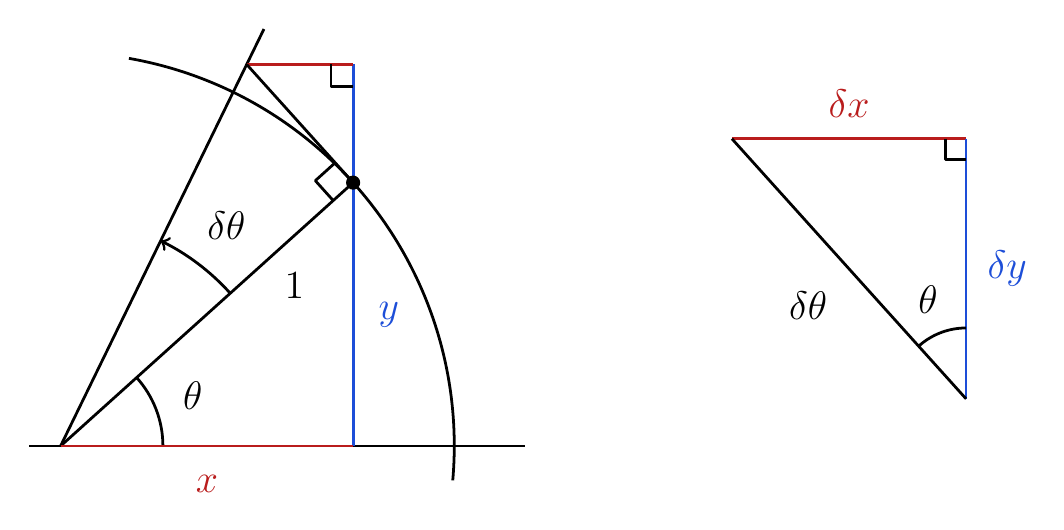
\begin{tikzpicture}[x=1mm, y=1mm]
  \def\R{50}\def\Th{42}\def\dTh{22}   % radius, angle, angular nudge (degrees)
  \def\k{2.2}                          % blow-up factor for the right panel
  \def\Xo{115}\def\Yo{6}                % bottom vertex of the blown-up triangle

  % legs of the tangent triangle: hypotenuse R*tan(dTheta), split by theta
  \pgfmathsetmacro{\hyp}{\R*tan(\dTh)}
  \pgfmathsetmacro{\dx}{\k*\hyp*sin(\Th)}
  \pgfmathsetmacro{\dy}{\k*\hyp*cos(\Th)}

  % ---------- left: the unit circle ------------------------------------------
  \coordinate (O) at (0,0);
  \coordinate (P) at (\Th:\R);
  \coordinate (T) at ({\Th+\dTh}:{\R/cos(\dTh)});   % tangent meets the outer ray
  \coordinate (C) at (P |- T);                      % corner of the small triangle
  \coordinate (X) at (P |- O);                      % foot on the axis

  \draw[hair, ink] (-4,0) -- ({\R+9},0);
  \draw[hair, ink] (-5:\R) arc[start angle=-5, end angle=80, radius=\R];
  \draw[edge, ink] (O) -- (P);
  \draw[hair, ink] (O) -- ({\Th+\dTh}:{\R/cos(\dTh)+5});

  % theta and its nudge at the origin
  \draw[hair, ink] (0:13) arc[start angle=0, end angle=\Th, radius=13];
  \node[ink] at ({\Th/2}:18) {$\theta$};
  \draw[hair, ink, ->] (\Th:29) arc[start angle=\Th, end angle={\Th+\dTh}, radius=29];
  \node[ink] at ({\Th+\dTh/2}:35) {$\delta\theta$};
  \node[ink] at (34.4:36) {$1$};

  % the sides that the nudge moves: y (and its increment) share one vertical line
  \draw[edge, figblue] (X) -- (C);
  \draw[edge, figred]  (O) -- (X);
  \draw[edge, figred]  (C) -- (T);
  \draw[edge, ink]     (P) -- (T);

  % right angles: radius vs. tangent at P, and the corner of the small triangle
  \draw[hair, ink] (P) ++(222:3.4) -- ++(132:3.4) -- ++(42:3.4);
  \draw[hair, ink] (C) ++(-2.8,0) -- ++(0,-2.8) -- ++(2.8,0);
  \fill[ink] (P) circle (0.9);

  \node[below, text=figred]  at ({\R*cos(\Th)/2},-2.5) {$x$};
  \node[right, text=figblue] at ({\R*cos(\Th)+2},{\R*sin(\Th)/2}) {$y$};

  % ---------- right: the same triangle, enlarged -----------------------------
  \coordinate (Pb) at (\Xo,\Yo);
  \coordinate (Cb) at (\Xo,{\Yo+\dy});
  \coordinate (Tb) at ({\Xo-\dx},{\Yo+\dy});

  \draw[edge, figred]  (Cb) -- (Tb);
  \draw[edge, figblue] (Cb) -- (Pb);
  \draw[edge, ink]     (Tb) -- (Pb);
  \draw[hair, ink] (Cb) ++(-2.6,0) -- ++(0,-2.6) -- ++(2.6,0);

  \draw[hair, ink] ([shift=(90:9)]Pb) arc[start angle=90, end angle={90+\Th}, radius=9];
  \node[ink] at ([shift={({90+\Th/2}:13.5)}]Pb) {$\theta$};

  \node[above, text=figred]  at ({\Xo-\dx/2},{\Yo+\dy+1.5}) {$\delta x$};
  \node[right, text=figblue] at ({\Xo+1.5},{\Yo+\dy/2}) {$\delta y$};
  % delta-theta label: midpoint of the hypotenuse, pushed out along its normal
  \node[ink] at ({\Xo-\dx/2-7*cos(\Th)},{\Yo+\dy/2-7*sin(\Th)}) {$\delta\theta$};
\end{tikzpicture}
\end{document}
